%% LyX 2.0.4 created this file.  For more info, see http://www.lyx.org/.
%% Do not edit unless you really know what you are doing.
\documentclass[english,annual]{acmsiggraph}
\usepackage[T1]{fontenc}
\usepackage[latin9]{inputenc}
\usepackage{amssymb}
\usepackage{graphicx}

\makeatletter
%%%%%%%%%%%%%%%%%%%%%%%%%%%%%% User specified LaTeX commands.
% for the following cases use the listed document class option:
% [annual] - Technical paper accepted for presentation at the ACM SIGGRAPH 
%   or SIGGRAPH Asia annual conference.
% [sponsored] - Short or full-length technical paper accepted for 
%   presentation at an event sponsored by ACM SIGGRAPH
%   (but not the annual conference Technical Papers program).
% [abstract] - A one-page abstract of your accepted content
%   (Technical Sketches, Posters, Emerging Technologies, etc.). 
%   Content greater than one page in length should use the "[sponsored]"
%   parameter.
% [preprint] - A preprint version of your final content.
% [review] - A technical paper submitted for review. Includes line
%   numbers and anonymization of author and affiliation information.

% When you submit your paper for review, please use the \TOGonlineID''
% command to include the online ID value assigned to your paper by the
% submission management system. Replace '45678' with the value you were
% assigned.
\TOGonlineid{45678}

% If you are preparing a preprint of your accepted paper, and your paper
% will be published in an issue of the ACM "Transactions on Graphics''
% journal, replace the "0'' values in the commands below with the correct
% volume and number values for that issue - you'll get them before your
% final paper is due.
\TOGvolume{0}
\TOGnumber{0}

% The TOGarticleDOI' command accepts the DOI information provided to you
% during production, and which makes up the URLs which identifies the ACM
% article page and direct PDF link in the ACM Digital Library.
% Replace "1111111.2222222'' with the values you are given.
\TOGarticleDOI{1111111.2222222}

% If you would like to include links to personal repositories for auxiliary
% material related your research contribution, you may use one or more of
% these commands to define an appropriate URL. The "\TOGlinkslist'' command
% found just before the first section of your document will add hyperlinked
% icons to your document, in addition to hyperlinked icons which point to
% the ACM Digital Library article page and the ACM Digital Library-held PDF.
\TOGprojectURL{}
\TOGvideoURL{}
\TOGdataURL{}
\TOGcodeURL{}

% Paper title.
\title{Curvature Enhance with Laplacian Operator for Hybrid Quad/Triangle Meshes}

% Author and Affiliation (single author).
%\author{Name \thanks{e-mail: name@unknown.uu}\\ Research Institute}

% Author and Affiliation (multiple authors).
\author{Alexander Pinzon\thanks{e-mail: apinzonf@gmail.com}\\ Cimalab Research Group %
\and Eduardo Romero\thanks{e-mail:edromero@unal.edu.co}\\Cimalab Research Group}
%\and Ton Roosendaal\thanks{e-mail:ton@blender.org}\\ Blender CEO}

% The ``pdfauthor'' command accepts the authors of the work,
% comma-delimited, and adds this information to the PDF metadata.
\pdfauthor{Alexander Pinzon, Eduardo Romero, Ton Roosendaal}

% Keywords that describe your work.
\keywords{laplacian smooth, curvature, sculpting, subdivision surface}

\makeatother

\usepackage{babel}
\begin{document}







\teaser{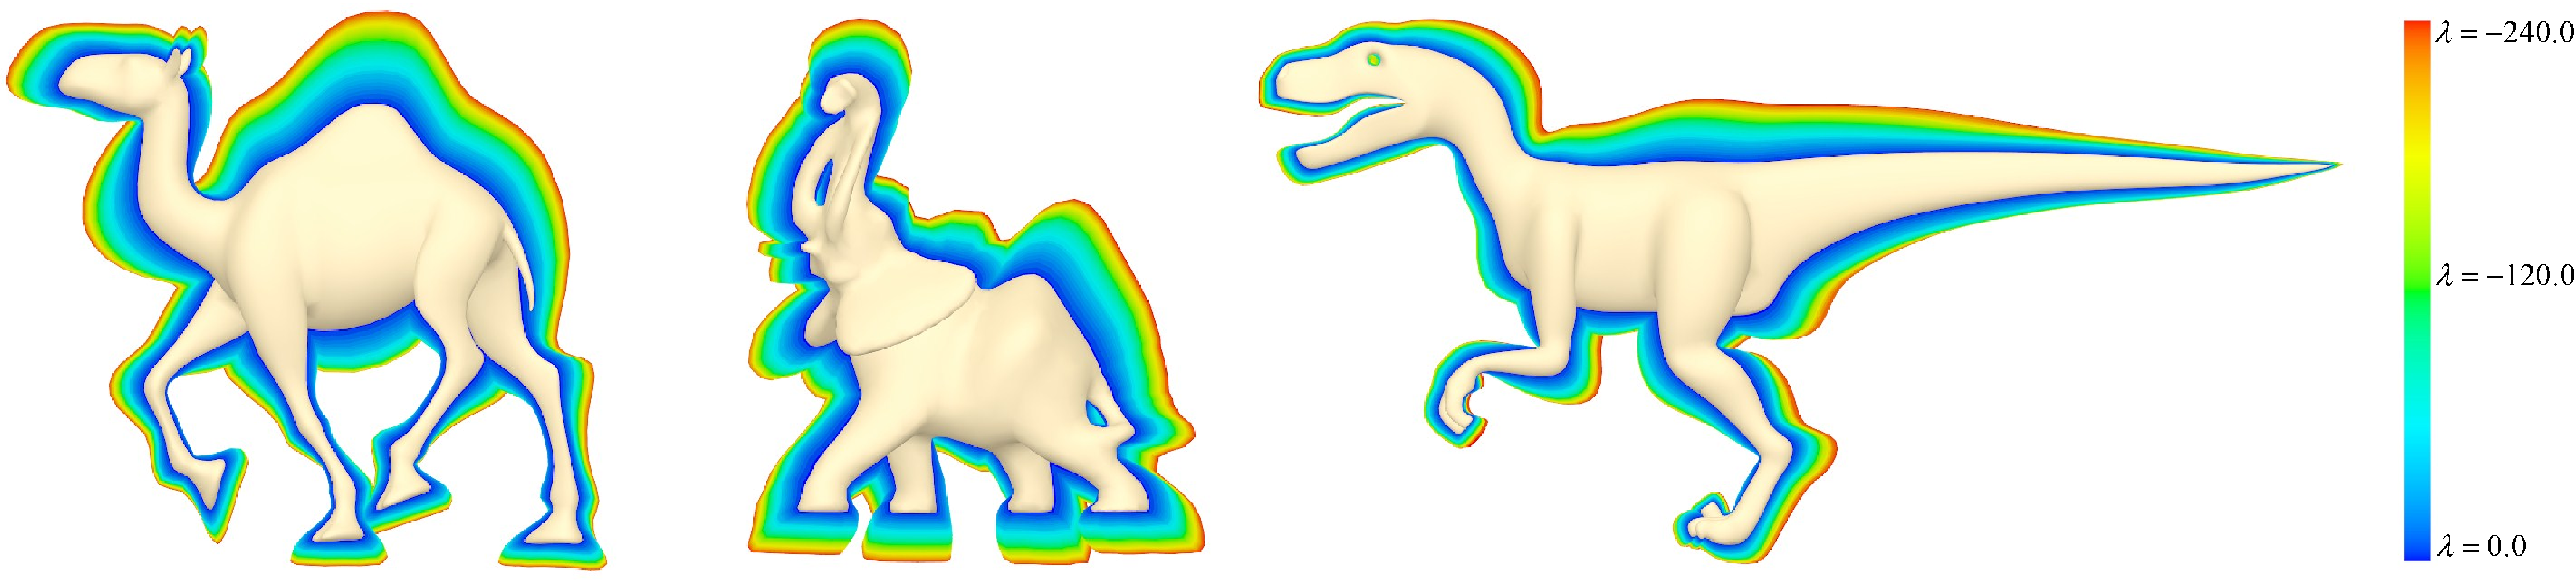
\includegraphics[width=1\textwidth]{images/spectrum} \caption{\label{fig:Spectrum}A set of 48 successive curvature enhance shapes,
from $\lambda=0.0$ in blue to $\lambda=-240.0$ in red, with steps
of $-5.0$.}
}

\maketitle
\maketitle 
\begin{abstract}
This paper proposes a novel method for modeling polygonal mesh using
curvature enhancing. This method use our extension of Laplace Beltrami
operator for hybrid quad/triangle meshes to enhance global curvature
in the model. This work present a novel applications of curvature
enhancement in sculpting and modeling with subdivision surfaces and
weight vertex groups. We show a series of graphics examples that demonstrate
the quality, predictability and flexibility of our results in a real
production environment with software blender.
\end{abstract}

\begin{CRcatlist}
\CRcat{I.3.5}{Computer Graphics}{Computational Geometry and Object Modeling
}{Modeling packages}
\end{CRcatlist}
\keywordlist

\TOGlinkslist

\copyrightspace


\section{Introduction}

Over the last years have been developed novel techniques of modeling
that can generate a variety of shapes to look natural and realistic
\cite{Botsch2006}. Editing techniques have evolved from affine transformations
to advanced tools like sculpting \cite{Coquillart1990,Galyean1991,Stanculescu2011},
editing and creation from sketches \cite{Igarashi1999,Gonen2012},
complex interpolation techniques \cite{Sorkine2004,Zhou2005}, among
others.

Traditional methods for smooth surfaces from coarse geometry like
Catmull-Clark have been widely developed \cite{Catmull1978,Stam1998},
these works generalize uniform B-cubic splines knot insertion to meshes,
some of them add control of the results with the use of creases to
produce sharp edges \cite{DeRose1998}, or the modification of weights
on the vertices that control locally the zone of influence \cite{Biermann2000},
instead our method performs a feature enhancement of the model allowing
parameterize the curvature of the surface creating a family of different
versions of the same object preserving detail and realistic natural
look of the original model. 

Many types of brushes have been developed to sculpt meshes, brushes
that perform inflation lose detail when inflating the vertices \cite{Stanculescu2011},
our method allows inflation of the mesh vertices moving in the opposite
direction to the curvature preserving the shape and sharp features
of the model.

This work is organized as follows: In the section \ref{sub:1.1-Related-work}
show works related to the Laplacian mesh processing, digital sculpting,
and offsetting methods for polygonal meshes; In the section \ref{sec:Laplacian-Smooth}
we describe the theoretical framework of the Laplacian operator for
polygon meshes; In the section \ref{sec:Proposed-Method} we present
our proposed method for curvature enhancement and applications on
subdivision surfaces and sculpting; Lastly some results are shown
in graphic examples of Laplacian operator for hybrid quad/triangle
meshes. Also shows some results of curvature enhancement applications
in sculpting, subdivision and modeling methods.

\textbf{Contributions} Our work present an extension of the Laplace
Beltrami operator for hybrid quad/triangle meshes representing a larger
spectrum of mesh that works with today eliminating the need for preprocessing
and allows the preservation of the original topology. With this operator
we proposed a method to generate family of parameterized shapes, in
a robust and predictable way. Our method enable to customization of
smoothness and curvature obtained during subdivision surfaces process.
We proposed a new brush for enhance silhouette features of mesh in
modeling and sculpting.


\section{Related work\label{sub:1.1-Related-work}}

Many tools have been developed for modeling based on Laplacian mesh
processing. Thanks to the kindness of the Laplacian operator these
tools have in common the need for preservation of the geometric details
of the surface for the different processes such as: free-form deformation,
fusion, morphing and other applications \cite{Sorkine2004}. 

Methods for offset polygon meshes based on the curvature defined by
the Laplace Beltrami operator have been developed. These methods allow
adjusting shape offset by a constant distance with high enough precision
to minimize Hausdorf error. The problem with these methods is the
loss of detail caused by smoothing, which depends on the size of the
offset \cite{Zhuo2012}. In volumetric approaches on computing the
offset boundary that are based on distance field computation in point-based
representation, this methods the topology of the offset model can
be different from that the original geometry \cite{Chen2011}.

\cite{Gal2009} proposes automatic features detection and shape edition
with feature inter-relationship preservation. In analysis step they
define salient surface features how ridges and valleys with base on
first and second order curvature derivatives \cite{Ohtake2004}, and
angle-based threshold. In feature characterization step the curves
are classified by several properties as planar or non-planar, approximated
by line, circle or ellipse shapes, and so on. In edit step the user
define initial change over several feature and then this edit is propagated
over other features with base in your inter-relationships. This method
works fine with objects that have sharp edges composed of basic geometric
shapes such as lines, circles or ellipses but this method has difficulties
when models are smoother with organic forms and cannot find the features
to edit and preserve.

Digital sculpting is divided into two principal methods: based on
polygonal methods and voxel grids-based methods. Brushes for inflate
operations in polygonal methods only depends on the normal at each
vertex \cite{Stanculescu2011}, in grids-based some operations permit
add or remove voxels and then have that processing isosurfaces from
volume to produce polygonal meshes representation \cite{Galyean1991}.
The problem whit this type of operations is the difficult to maintain
surface details during larger scale deformation.


\section{Laplacian Smooth\label{sec:Laplacian-Smooth}}

\begin{figure*}[t]
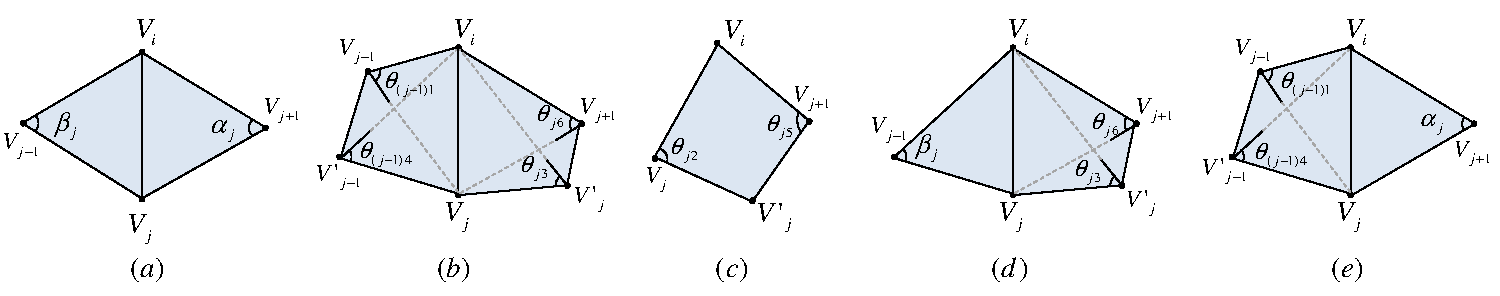
\includegraphics[width=1\textwidth]{images/beltrami}

\caption{\label{fig:LBO-basic-5-TQ}The 5 basic triangle-quad cases with common
vertex $V_{i}$ and the relationship with $V_{j}$ and $V_{j}^{\prime}$.
(a) Two triangles {[}Desbrun 1999{]}. (b) (c) Two quads and one quad
{[}Xiong 2011{]}. (d) (e) Triangles and quads (TQLBO).}
\end{figure*}


The Laplacian Smooth techniques allows you to reduce noise on a mesh's
surface with minimal changes on its shape. Computer graphics objects
which have been reconstructed from real world, contain undesirable
noise. A Laplacian smoothing removes undesirable noise while still
preserves desirable geometry as well as the shape of the original
model. 

The functional used in many Laplacian smoothing approach to constrain
energy minimization is based on a total curvature of a surface $S$.

\begin{equation}
E\left(S\right)=\int_{S}\kappa_{1}^{2}+\kappa_{2}^{2}dS\label{eq:total_cuarvature_integral}
\end{equation}


Where $\kappa_{1}$ and $\kappa_{2}$ are the two principal curvatures
of the surface $S$.


\subsection{Gradient of Voronoi Area}

\begin{figure}[h]
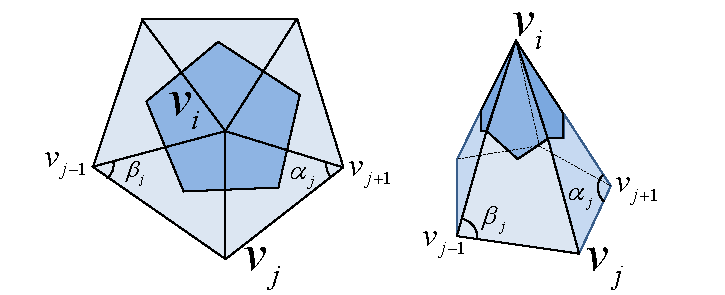
\includegraphics[width=1\columnwidth]{images/voronoi_region}

\caption{\label{fig:voronoi_region}Area of Voronoi region around $v_{i}$
in dark blue.\protect \\
 $v_{j}$ 1-ring neighbors around $v_{i}$. $\alpha_{j}$ and $\beta_{j}$
opposite angles to edge $\protect\overrightarrow{v_{j}-v_{i}}$. }
\end{figure}


Consider a surface $S$ compound by a set of triangles around vertex
$v_{i}$. We can define the \textit{Voronoi region} of $v_{i}$ as
show in figure \ref{fig:voronoi_region}, The change in area produced
by move $v_{i}$ is named gradient of \textit{Voronoi region \cite{Pinkall1993,Desbrun1999,Meyer2003}.}

\begin{equation}
\nabla A=\frac{1}{2}\underset{j}{\sum}\left(\cot\alpha_{j}+\cot\beta_{j}\right)\left(v_{i}-v_{j}\right)\label{eq:eq_gradient_voronoi_area}
\end{equation}


If we normalize this gradient in equation (\ref{eq:eq_gradient_voronoi_area})
by the total area in 1-ring around $v_{i}$, we have the \textit{discrete
mean curvature normal} of a surface $S$ as shown in equation (\ref{eq:discrete_mean_curvature_normal}).

\begin{equation}
2\kappa\mathbf{n}=\frac{\nabla A}{A}\label{eq:discrete_mean_curvature_normal}
\end{equation}



\subsection{Laplace Beltrami Operator}

The \textit{Laplace Beltrami operator} LBO denoted $\triangle_{g}$
is used for measures mean curvature normal of the Surface $S$ \cite{Pinkall1993}. 

\begin{equation}
\triangle_{g}S=2\kappa\mathbf{n}\label{eq:def_LBO}
\end{equation}


The LBO has desirable features, one feature of the LBO is in direction
of surface area minimization, allowing us to minimize energy using
it on a total curvature of a surface $S$ at equation (\ref{eq:total_cuarvature_integral}).


\section{Proposed Method\label{sec:Proposed-Method}}

Our method allow the editing of geometric features using the curvature
enhancement and smoothing. Generating a parameterized family of shapes
using a set of vertices representing a coarse sketch of the desired
model. Our approach can be mixed with traditional or uniform subdivision
surfaces methods and is iterative and converges towards a continuous
and smooth version of the original model. 

Unlike other methods, our method allows to use mixed arbitrary types
of mesh representation as triangles and quads, exploiting the basic
geometrical relationships facilitating and ensuring convergence of
the algorithm and similar shapes consistent with the original shape
against the other methods. 

Our method allows the use of soft constraints weighting the effect
of smoothing at each vertex based on a normalized weight, the weights
are assigned to the control vertices of the original mesh or. The
weights of the new vertices resulting from the subdivisions are calculated
by interpolation, allowing to modify the behavior of the method on
exact regions of the original model.

Our approach contain an extension of the Laplace Beltrami operator
for meshes composed by triangles and quads. Using meshes composed
by triangles and quads has been increasing in recent years due to
the flexibility of modeling tools as Blender 3D \cite{blender}. Today
many artists manually connecting vertices such that its edition allows
simplest way to perform animation processes and interpolation \cite{Mullen2007}.
For these reasons it is very important to develop an operator that
allows working with this type of mesh immediately, eliminating the
need to preprocessing the mesh to convert to triangles and losing
the original design made by users.


\subsection{Laplace Beltrami Operator for Hybrid Quad/Triangle Meshes TQLBO\label{sub:Laplace-Beltrami-operator}}

Given a mesh $M=\left(V,Q,T\right)$, with vertices $V$, quads $Q$,
triangles $T$.

The area of $1$-ring neighborhood ($N_{1}$) with shared face quad
or triangle to vertex $v_{i}$ in $M$ is.

\begin{center}
$A\left(v_{i}\right)=A\left(Q_{N_{1}\left(v_{i}\right)}\right)+A\left(T_{N_{1}\left(v_{i}\right)}\right)$.
\par\end{center}

\begin{figure}[h]
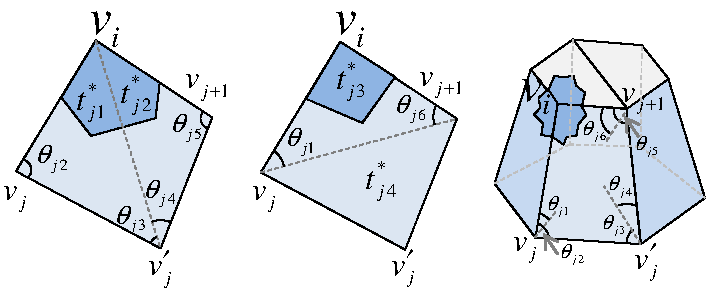
\includegraphics[width=1\columnwidth]{images/quad_xiong}

\caption{\label{fig:quad_xiong}$t_{j1}^{*}\equiv\vartriangle v_{i}v_{j}v_{j}^{\prime},\, t_{j2}^{*}\equiv\vartriangle v_{i}v_{j}^{\prime}v_{j+1},\, t_{j3}^{*}\equiv\vartriangle v_{i}v_{j}v_{j+1}$
Triangulations of the quad with common vertex $v_{i}$ proposed by
{[}Xiong 2011{]} to define Mean LBO.}
\end{figure}


Applying the mean average area according to \cite{Xiong2011} of all
possible triangulations for each quad to $A\left(Q_{N_{1}\left(v_{i}\right)}\right)$
as show in figure \ref{fig:quad_xiong}.

\begin{center}
$A\left(v_{i}\right)=\frac{1}{2^{m}}\overset{m}{\underset{j=1}{\sum}}2^{m-1}A\left(q_{j}\right)+\overset{r}{\underset{k=1}{\sum}}A\left(t_{k}\right)$
\par\end{center}

Where $q_{1},q_{2},...,q_{j},...,q_{m}\in Q_{N_{1}\left(v_{i}\right)}$
and $t_{1},t_{2},...,t_{k},...,t_{r}\in T_{N_{1}\left(v_{i}\right)}$.

\begin{equation}
A\left(v_{i}\right)=\frac{1}{2}\overset{m}{\underset{j=1}{\sum}}\left[A\left(t_{j1}^{*}\right)+A\left(t_{j2}^{*}\right)+A\left(t_{j3}^{*}\right)\right]+\overset{r}{\underset{k=1}{\sum}}A\left(t_{k}\right)\label{eq:area_1_ring_triangles_quads}
\end{equation}


Applying the gradient operator to (\ref{eq:area_1_ring_triangles_quads}).

\begin{equation}
\nabla A\left(v_{i}\right)=\frac{1}{2}\overset{m}{\underset{j=1}{\sum}}\left[\nabla A\left(t_{j1}^{*}\right)+\nabla A\left(t_{j2}^{*}\right)+\nabla A\left(t_{j3}^{*}\right)\right]+\overset{r}{\underset{k=1}{\sum}}\nabla A\left(t_{k}\right)\label{eq:EqGrad}
\end{equation}


According to (\ref{eq:eq_gradient_voronoi_area}), we have.

\begin{center}
$\nabla A\left(t_{j1}^{*}\right)=\frac{\cot\theta_{j3}\left(v_{j}-v_{i}\right)+\cot\theta_{j2}\left(v_{j}^{\prime}-v_{i}\right)}{2}$
\par\end{center}

\begin{center}
$\nabla A\left(t_{j2}^{*}\right)=\frac{\cot\theta_{j5}\left(v_{j}^{\prime}-v_{i}\right)+\cot\theta_{j4}\left(v_{j+1}-v_{i}\right)}{2}$
\par\end{center}

\begin{center}
$\nabla A\left(t_{j3}^{*}\right)=\frac{\cot\theta_{j6}\left(v_{j}-v_{i}\right)+\cot\theta_{j1}\left(v_{j+1}-v_{i}\right)}{2}$
\par\end{center}

\begin{center}
$\nabla A\left(t_{k}\right)=\frac{\cot\alpha_{k}\left(v_{k}-v_{i}\right)+\cot\beta_{k+1}\left(v_{k+1}-v_{i}\right)}{2}$
\par\end{center}

All triangles and quads configurations of the 1-ring neighborhood
faces adjacent to $v_{i}$ can be simplified in five simple cases
how show in figure \ref{fig:LBO-basic-5-TQ}.

Then according to equation (\ref{eq:discrete_mean_curvature_normal}),
(\ref{eq:def_LBO}), and five simple cases defined in figure \ref{fig:LBO-basic-5-TQ}
the TQLBO (Triangle-Quad LBO) of $v_{i}$ is.

\begin{equation}
\triangle_{g}\left(v_{i}\right)=2\kappa\mathbf{n}=\frac{\nabla A}{A}=\underset{v_{j}\in N_{1}\left(v_{i}\right)}{\frac{1}{2A}\sum}w_{ij}\left(v_{j}-v_{i}\right)
\end{equation}


\begin{equation}
w_{ij}=\begin{cases}
\left(\cot\alpha_{j}+\cot\beta_{j}\right) & \mbox{case }\mathit{a.}\\
\frac{1}{2}\left(\cot\theta_{\left(j-1\right)1}+\cot\theta_{\left(j-1\right)4}+\cot\theta_{j3}+\cot\theta_{j6}\right) & \mbox{case \ensuremath{\mathit{b}}.}\\
\left(\cot\theta_{j2}+\cot\theta_{j5}\right) & \mbox{case \ensuremath{\mathit{c}}.}\\
\frac{1}{2}\left(\cot\theta_{j3}+\cot\theta_{j6}\right)+\cot\beta_{j} & \mbox{case \ensuremath{\mathit{d}}.}\\
\frac{1}{2}\left(\cot\theta_{\left(j-1\right)1}+\cot\theta_{\left(j-1\right)4}\right)+\cot\alpha_{j} & \mbox{case \ensuremath{\mathit{e}}.}
\end{cases}\label{eq:TQLBO_wij}
\end{equation}


We define a Laplacian operator as a matrix equation

\begin{equation}
L\left(i,j\right)=\begin{cases}
-\frac{1}{2A_{i}}w_{ij} & \mbox{if }j\in N\left(v_{i}\right)\\
\frac{1}{2A_{i}}\underset{j\in N\left(v_{i}\right)}{\sum}w_{ij} & \mbox{if }i=j\\
0 & \mbox{otherwise}
\end{cases}\label{eq:TQLBO_Simple_Matrix}
\end{equation}


Where $L$ is the $n\times n$ matrix, $n$ is the number of vertices
of a given mesh $M$, $w_{ij}$ is the TQLBO defined in equation (\ref{eq:TQLBO_wij}),
$N\left(v_{i}\right)$ is the 1-ring neighborhood with shared face
to $v_{i}$, $A_{i}$ is the ring area around $v_{i}$.

Normalized version of the TQLBO as a matrix equation

\begin{equation}
L\left(i,j\right)=\begin{cases}
-\frac{w_{ij}}{\underset{j\in N\left(v_{i}\right)}{\sum}w_{ij}} & \mbox{if }j\in N\left(v_{i}\right)\\
\delta_{ij} & \mbox{otherwise}
\end{cases}\label{eq:TQLBO-Normalized_Matrix}
\end{equation}


Where $\delta_{ij}$ being the Kronecker delta function.


\subsection{Curvature Enhancing\label{sub:Curvature-Enhancing}}

\begin{figure*}[t]
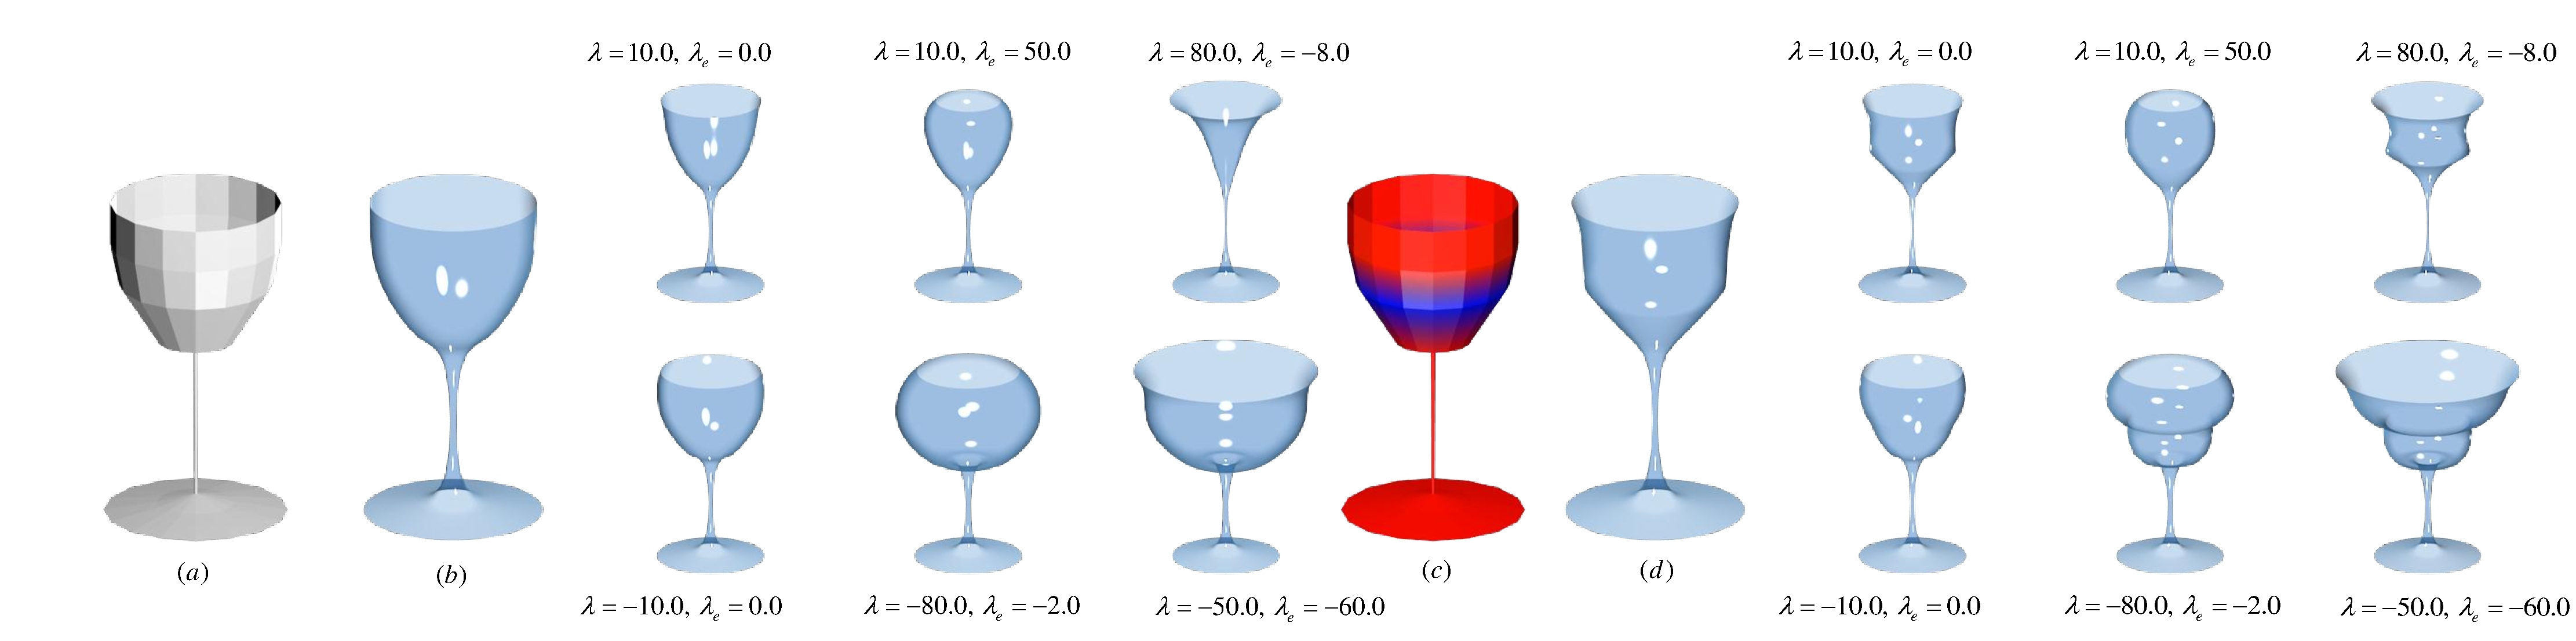
\includegraphics[width=1\textwidth]{images/teaser_cup}

\caption{\label{fig:Subdivision-Cups} Family of cups generated with our method
from coarse model to enhancing the curvature obtained from Catmull-Clark
Subdivision and the use of constraints over coarse model with weight
vertex group in red.}


\end{figure*}


The curvature enhancing use the change produced by Laplacian smoothing
in the inverse direction of the curvature flow for moves the vertices
in the portions of the mesh with most curvature. In this equation
we use a diffusion process:

\begin{center}
$\frac{\partial V}{\partial t}=\lambda L\left(V\right)$ 
\par\end{center}

For solve the equation above we use implicit integration and a normalized
version of TQLBO matrix.

\begin{equation}
\left(I-\left|\lambda dt\right|W_{p}L\right)V^{\prime}=V^{t}\label{eq:Lineal_System_with_wp}
\end{equation}


\begin{center}
$V^{t+1}=V^{t}+\mbox{sign}\left(\lambda\right)\left(V^{\prime}-V^{t}\right)$
\par\end{center}

The vertices $V^{t+1}$are enhance along their inverse curvature normal
directions by solving this simple linear system: $Ax=b$, where $A=I-\left|\lambda dt\right|W_{p}L$,
$L$ is the Normalized TQLBO defined in the equation (\ref{eq:TQLBO-Normalized_Matrix}),
$x=V^{\prime}$ are the smoothing vertices, $b=V^{t}$ are the actual
vertices positions, $W_{p}$ is a diagonal matrix with weight vertex
group, $\mbox{sign}\left(x\right)$ is the sign function, and $\lambda dt$
is the enhance factor that support negative and positive values, negative
for enhancing positive for smoothing. 

At the borders of the meshes that are not closed, you can not calculate
the curvature, for that reason we use the scale-dependent operator
proposed by \cite{Desbrun1999}.

Our method was designed for use with weight vertex groups to specify
the degree of impact on the solution, the weights vary between $0$
and $1$ with a value of $0$ makes no changes and with values 1 applies
the total change. The weights modifying influence zones where the
Laplacian is applied as shown in the equation \ref{eq:Lineal_System_with_wp}.
The weights on each vertex will produce a different solution for that
reason are put before obtaining the solution of the linear system.
Families of shapes that are generated may change substantially with
the weights of specific control points.

The model volume increases as the lambda is most negative, this can
be countered by a simple method of preserving volume. In \cite{Desbrun1999}
present a simple method to resize the mesh but have a problem the
model suffer large displacements with $\lambda<-1.0$ or perform multiple
iterations. We propose the following solution: If we have $v_{i}^{t+1}$
is a mesh vertex of $V^{t+1}$ in the $t+1$ iteration, we define
$\overline{v}$ as:

\begin{center}
$\overline{v}=\frac{1}{n}\underset{v_{i}\in V}{\sum}v_{i}$, 
\par\end{center}

$\overline{v}$ is the center of the mesh, $vol_{ini}$ is an initial
volume, and $vol_{t+1}$ is the volume at the iteration $t+1$, then
we have that scale factor for resize the volume is

\begin{center}
$\beta=\left(\frac{vol_{ini}}{vol_{t+1}}\right)^{\frac{1}{3}}$
\par\end{center}

and the new vertices positions are:

\begin{center}
$v_{i\, new}^{t+1}=\beta\left(v_{i}^{t+1}-\overline{v}\right)+\overline{v}$
\par\end{center}


\subsection{Sculpting\label{sub:Sculpting}}

\begin{figure*}[t]
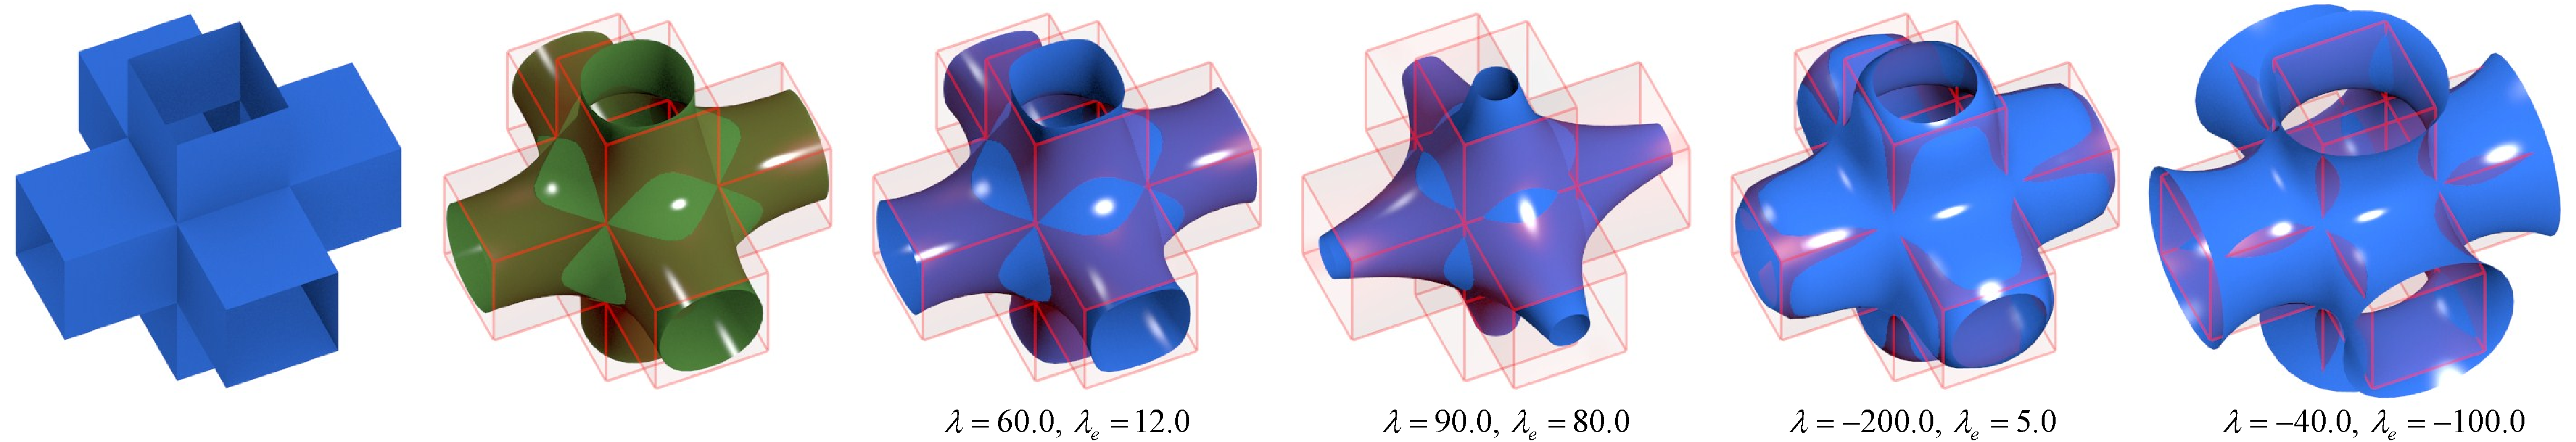
\includegraphics[width=1\textwidth]{images/cruz_lambda4}

\caption{\label{fig:Catmull_Clark}Left: Original Model, in green color model
with Catmull-Clark Subdivision. Models with Laplacian smoothing: $\lambda=60.0$,
$\lambda_{e}=12.0$ and $\lambda=90.0$, $\lambda_{e}=80.0$. Models
first filter with Laplacian smoothing $\lambda=60.0$, $\lambda_{e}=12.0$
and before applied curvature enhancing: $\lambda=-200.0$, $\lambda_{e}=12.0$
and $\lambda=-40.0$, $\lambda_{e}=-100.0$.}
\end{figure*}


We design a new brush that allows enhancement of the curvatures of
a polygon mesh in real time. Our brush work well with the stroke method
\textsl{Drag Dot} developed in the sculpt mode in Blender \cite{blender}
which allows you to preview the change that occurs in the model until
you release the mouse button or tablet, also enable moves the mouse
over the model to fit exactly where you want to perform the enhancement
of the curvature.

Brushes that perform similar work as inflate can create distortions
in the mesh and can also produce self-intersections of the mesh, as
this brushes only moves the vertices along the normal and does not
take into account the global information. Whereas our method look
for the best way to make inflation while keeping the global curvature
for preserving the shape and sharp features of the model.

Our method simplifies the work required for the enhancement, which
would be to use some different brushes for inflating and some other
to soften and styling. With our enhanced brush can be performed in
one step.

For the real-time work brush is necessary that the matrix is constructed
with the vertices that are within the radius defined by the user involvement,
which dramatically reduces the size of the matrix to be processed,
the center of this sphere depends on the place where the user clicks
on the canvas and three-dimensional mesh place where the click is
projected. 

Furthermore special handling is necessary with the vertices are at
the boundary of which have neighbors that are not within the radius
of impact, these vertices must be marked as boundary and not the curvature
calculated for them, but must be present in the matrix to allow the
vertices that have all their neighbors within the selection radius
to calculate correctly the curvature, this change allows the results
to be much smoother on the border. The Laplacian matrix for sculpt
mode as a matrix equation.

\begin{center}
$L\left(i,j\right)=\begin{cases}
-\frac{w_{ij}}{\underset{j\in N\left(v_{i}\right)}{\sum}w_{ij}} & \mbox{if }\left\Vert v_{i}-u\right\Vert <r\wedge\left\Vert v_{j}-u\right\Vert <r\\
0 & \mbox{if }\left\Vert v_{i}-u\right\Vert <r\wedge\left\Vert v_{j}-u\right\Vert \geq r\\
\delta_{ij} & \mbox{otherwise}
\end{cases}$
\par\end{center}

Where $v_{j}\in N\left(v_{i}\right)$, $u$ is the center of sphere
the radius $r$. Then the matrix should remove rows and columns of
vertices index that are not within the radius.


\subsection{Subdivision surfaces\label{sub:Subdivision-surfaces}}

The Catmull-Clark subdivision transformation is used to smooth a surface
as the limit of sequence of subdivision steps\cite{Stam1998}. This
method do a recursive subdivision transformation that refines the
model into a linear interpolation that is a approximate smooth surface.
The process of Catmull-Clark is govern by properties of B-spline curve
from multivariate spline theory\cite{Loop1987}. In many subdivision
surfaces methods Catmull-Clark, Loop so on, the smoothness of the
model is automatically guaranteed \cite{DeRose1998}. 

Catmull-Clark subdivision surface method generates smooth and continuous
models from a coarse model and produce results quickly due to the
simplicity of implementation, but with these methods is not easy to
make changes to the global curvature of the model. If we use Catmull-Clark
subdivision surfaces and curvature enhancement for modeling from coarse
models with few vertices can generate families of shapes with just
change a parameter, which would allow an artist to choose the model
of a similar set of options that best meets your needs without having
to change each one of the control vertices.

Our method allows the use of vertex weight paint over the control
points. The weights can be applied to the coarse model, then to perform
subdivision weights are interpolated, producing weights with smooth
changes in the zones of influence, so the curvature that is obtained
is much softer at those areas. Using vertex group weight and subdivision
surfaces is shown in figure \ref{fig:Subdivision-Cups}.c.

In the equation \ref{eq:Lineal_System_with_wp}, $W_{p}$ is a diagonal
matrix with weights corresponding to each vertex. The weights at each
vertex produce a different solution for this reason the matrix is
placed in the diffusion equation, as families that are generated may
change substantially with weighted of specific control points.


\section{Results\label{sec:Results}}

In this section we describe the results of our curvature enhance method
that used our extension of Laplace Beltrami operator for hybrid quad/triangle
meshes with several example models in figures \ref{fig:Spectrum},
\ref{fig:Subdivision-Cups}, \ref{fig:Catmull_Clark}, \ref{fig:TQLBO_test},
\ref{fig:camello_enhanced}, \ref{fig:Sculpt_Brush}, \ref{fig:Performance-sculpt},
\ref{fig:(a)Monkey}, \ref{fig:Animated_Camell}. We test the curvature
enhance with TQLBO method on a PC with AMD Quad-Core Processor @ 2.40
GHz and 8 GB RAM.

Figure \ref{fig:TQLBO_test} show the results when applying Laplace
Beltrami Operator TQLBO of equation (\ref{eq:TQLBO_Simple_Matrix})
in a model with a simple subdivision. In column (c) Laplacian smoothing
was applied to the model consists of only quads. In column (d) the
model was converted to triangles and then Laplacian smoothing was
applied. In column (e) the model is converted randomly some quads
into triangles and then Laplacian smoothing was applied, showing similar
results to those composed only of triangles or squares.

\begin{figure}
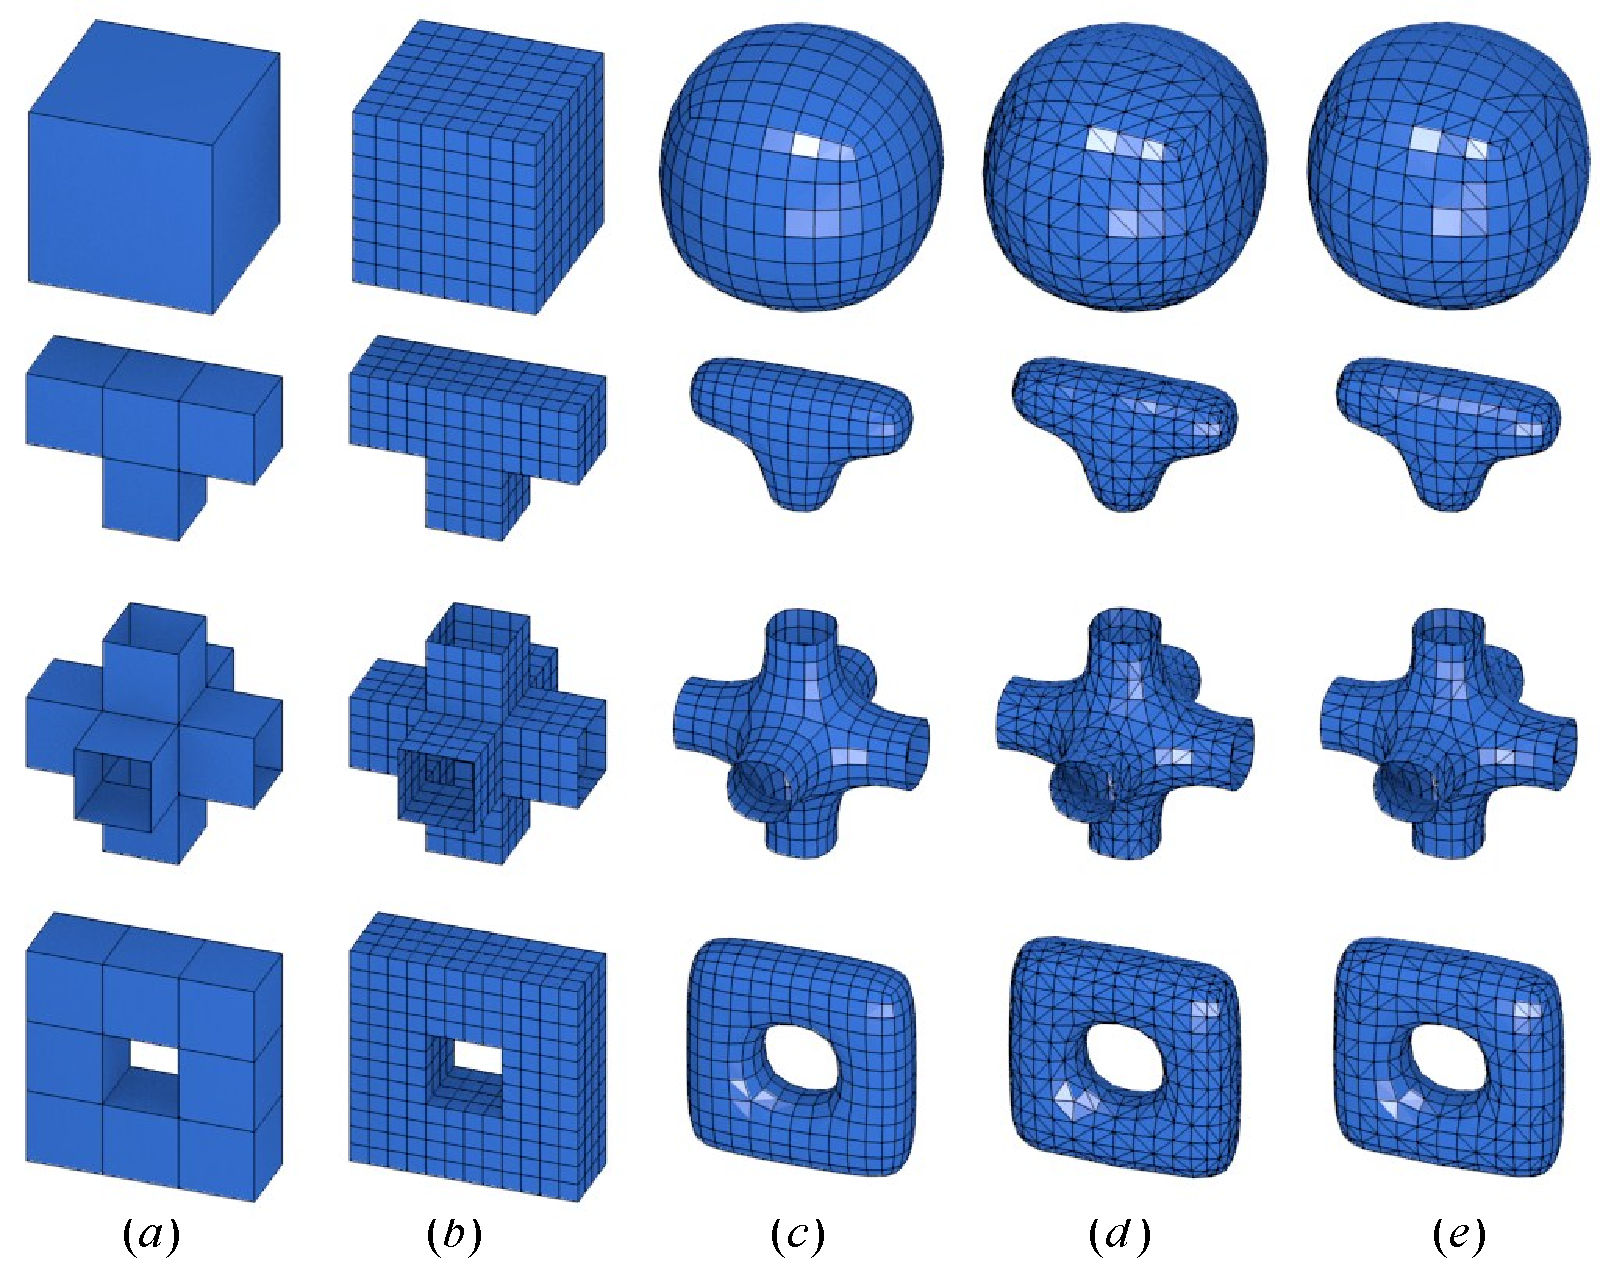
\includegraphics[width=1\columnwidth]{images/test_triangles_quads}

\caption{\label{fig:TQLBO_test}(a) Original Model. (b) Simple subdivision.
(c), (d) (e) Laplacian smoothing with $\lambda=7$ and 2 iterations:
(c) for triangles, (d) for quads, (e) for triangles and quads random
chosen.}
\end{figure}


Methods using Catmull-Clark subdivision surface and the enhancement
allows to modify the curvature that is obtained with the process of
subdivision as shown in figure \eqref{fig:Subdivision-Cups} this
test used a coarse model of a cup, after the model was performed subdivision
then was performed Laplacian smoothing and enhancement by modifying
the parameters $\lambda$ y $\lambda_{e}$ corresponding to the lambda
for rings and edges respectively. In figure \eqref{fig:Subdivision-Cups}.c,
\eqref{fig:Subdivision-Cups}.d shows also the use weight vertex groups
over coarse models with subdivision surfaces that allowed to generate
the weights for the new interpolated vertices, these new weights were
used for the enhancement obtained the 6 cups that are to the right
of the figure \eqref{fig:Subdivision-Cups}.d.

Laplacian smoothing applied with simple subdivision may produce results
similar to obtained with Catmull-Clark whose models are on average
equal triangles as shown in figure \ref{fig:Catmull_Clark} green
model and that obtained with Laplacian smoothing $\lambda=60.0$,
$\lambda_{e}=12.0$, but also can modify the curvature obtained after
applying Catmull-Clark as shown in the three columns to the right
of the figure \ref{fig:Catmull_Clark}.

Figure \ref{fig:camello_enhanced} show the generation of different
version of camel with the variation of parameter lambda. In the top
row you can see results of do curvature enhance over all model, as
the lambda becomes more negative curvature in this model makes close
in the concave parts and inflates on the convex parts as shown in
figure \ref{fig:Spectrum}. We use negative values to enhance model
silhouette features, among more negative the lambda, the model will
be further enhanced the silhouette features. In the bottom row of
the figure \ref{fig:camello_enhanced} can be observed using weighted
vertex groups, which allows you to specify which areas you want to
model enhancement, on the left is the enhancement of the legs of the
camel produces enhancement of organic aspect, also notes that the
border is not distorted and smooth in the union.

\begin{figure}
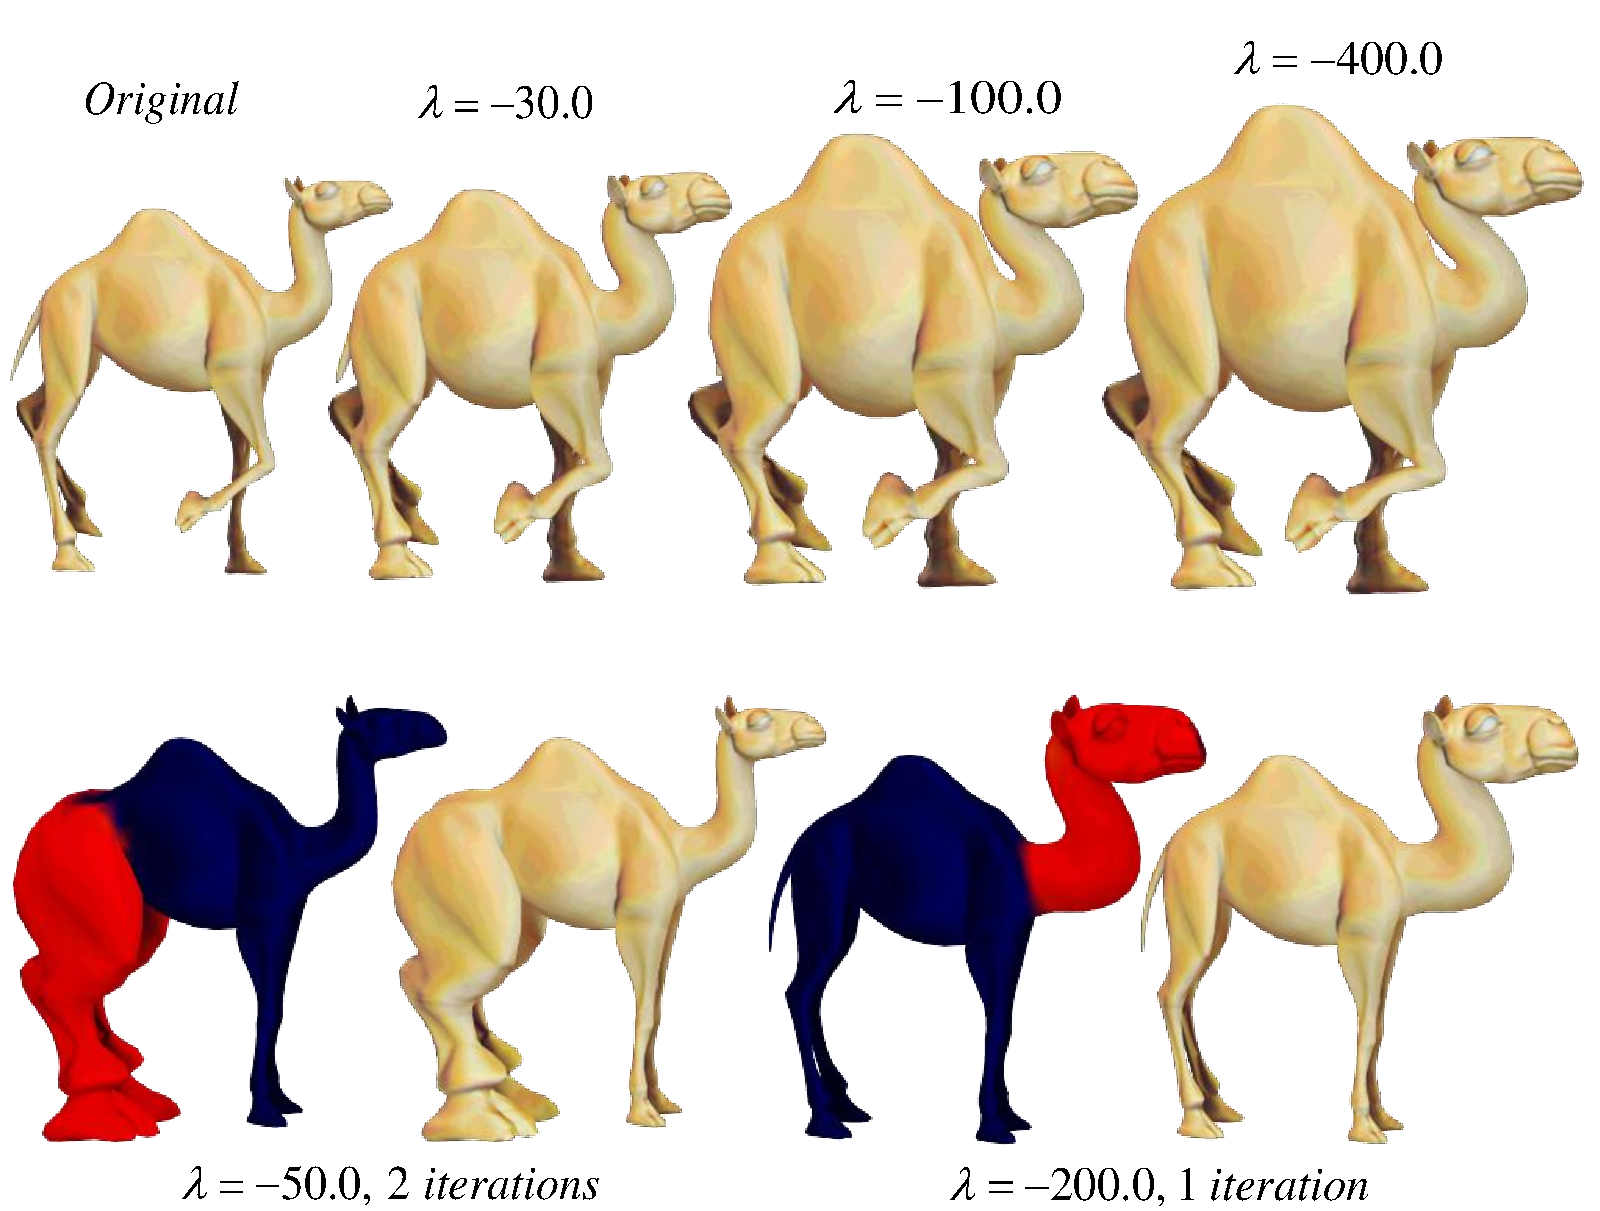
\includegraphics[width=1\columnwidth]{images/camello_enhanced2}

\caption{\label{fig:camello_enhanced}Top row: Original camel model in left.
Curvature enhancing with $\lambda=-30.0$, $\lambda=-100.0$, $\lambda=-400.0$.
Bottom row: Curvature enhancing with weight vertex group, $\lambda=-50.0$
and 2 iterations at legs, $\lambda=-200.0$ and 1 iteration in head
and neck.}
\end{figure}


Our method for enhancement of the silhouette features is predictable
and invariant under isometric transformations as those present in
some animations (see Figure \ref{fig:Animated_Camell}) in this animation
shows some poses of a camel doing a walk. In this animation the legs
and neck are the parts that enhancement is performed as shown in the
bottom left part of the figure \ref{fig:Animated_Camell}. Local modifications
produced by methods such as pose interpolation or animation rigging
not significantly affect the result as with camel legs in each sample
pose different flexion of the leg joints enhancement camel keeps flesh-like
shapes in the pattern produced original by the artist. This is due
to the diffusion process which is subjected to the mesh so that small
local changes are treated without significantly affecting global solution.
Our method is invariant of rotation, since depends solely the normal
field of the mesh, wish is invariant under global rotations. 

Figure \ref{fig:Sculpt_Brush} shows the use of curvature enhancement
brush for sculpting in real time. One pass was used with the brush
as shown in the figure with the blue and red radius. In the bottom
of the figure \ref{fig:Sculpt_Brush}.b shows how the camel leg self-intersecting
and looks like two bubbles stuck, so do the fingers on the bottom
of figure. Using silhouette features enhancement in figure \ref{fig:Sculpt_Brush}.c
we see better results because not lost the shape of the silhouette
and kept the details of the fingers and leg. Similar results can be
obtained by an artist but it would take several steps and the use
of several brushes with curvatures enhancement only takes one step.
With this new method can easily enhance organic features how muscles
during the sculpting process. In figure \ref{fig:Performance-sculpt}
we show the performance of curvature enhancement brush, in this experimet
we use three models with 12K, 40K and 164K vertices, this models were
sculpted with curvature enhance brush in eache step the brush sphere
contain a variable number of vertices for processing. The processing
time for 800 vertices in the camel paw (40k model) only take 0.1 seconds,
for 2600 vertices in leg and neck (model 40k) take 0.5 seconds, these
times are good, because usually an artist sculpts a model for parts,
and each part is represented by an average of about 3000 vertices
in the models we use.

We did tests with the Laplacian operator to equation (\ref{eq:TQLBO_Simple_Matrix})
and its normalized version equation (\ref{eq:TQLBO-Normalized_Matrix}),
the two produce similar results if the triangles that compose the
mesh are the same size on average , but the normalized version is
more stable and predictable because it is not divided by the area
of the ring which may be zero or very small and cause problems due
to floating point calculation errors as shown in figure \ref{fig:(a)Monkey}.c
bottom row in which the mesh is deformed because the TQLBO is susceptible
to the size of the triangle. The enhancement of curvature of the model
with the normalized Laplacian operator has a more regular behavior.
The model can deform in TQLBO normalized version with large lambdas>
400 intersects self, but produces no peaks observed with the TQLBO.
Figure \ref{fig:(a)Monkey} observed different results because the
area of the triangles in this model is not so regular triangles where
greater area enhancement is less (figure \ref{fig:(a)Monkey}.c skull),
and where the smaller triangles are produced greater enhancement (figure
\ref{fig:(a)Monkey}.c chin).

\begin{figure}
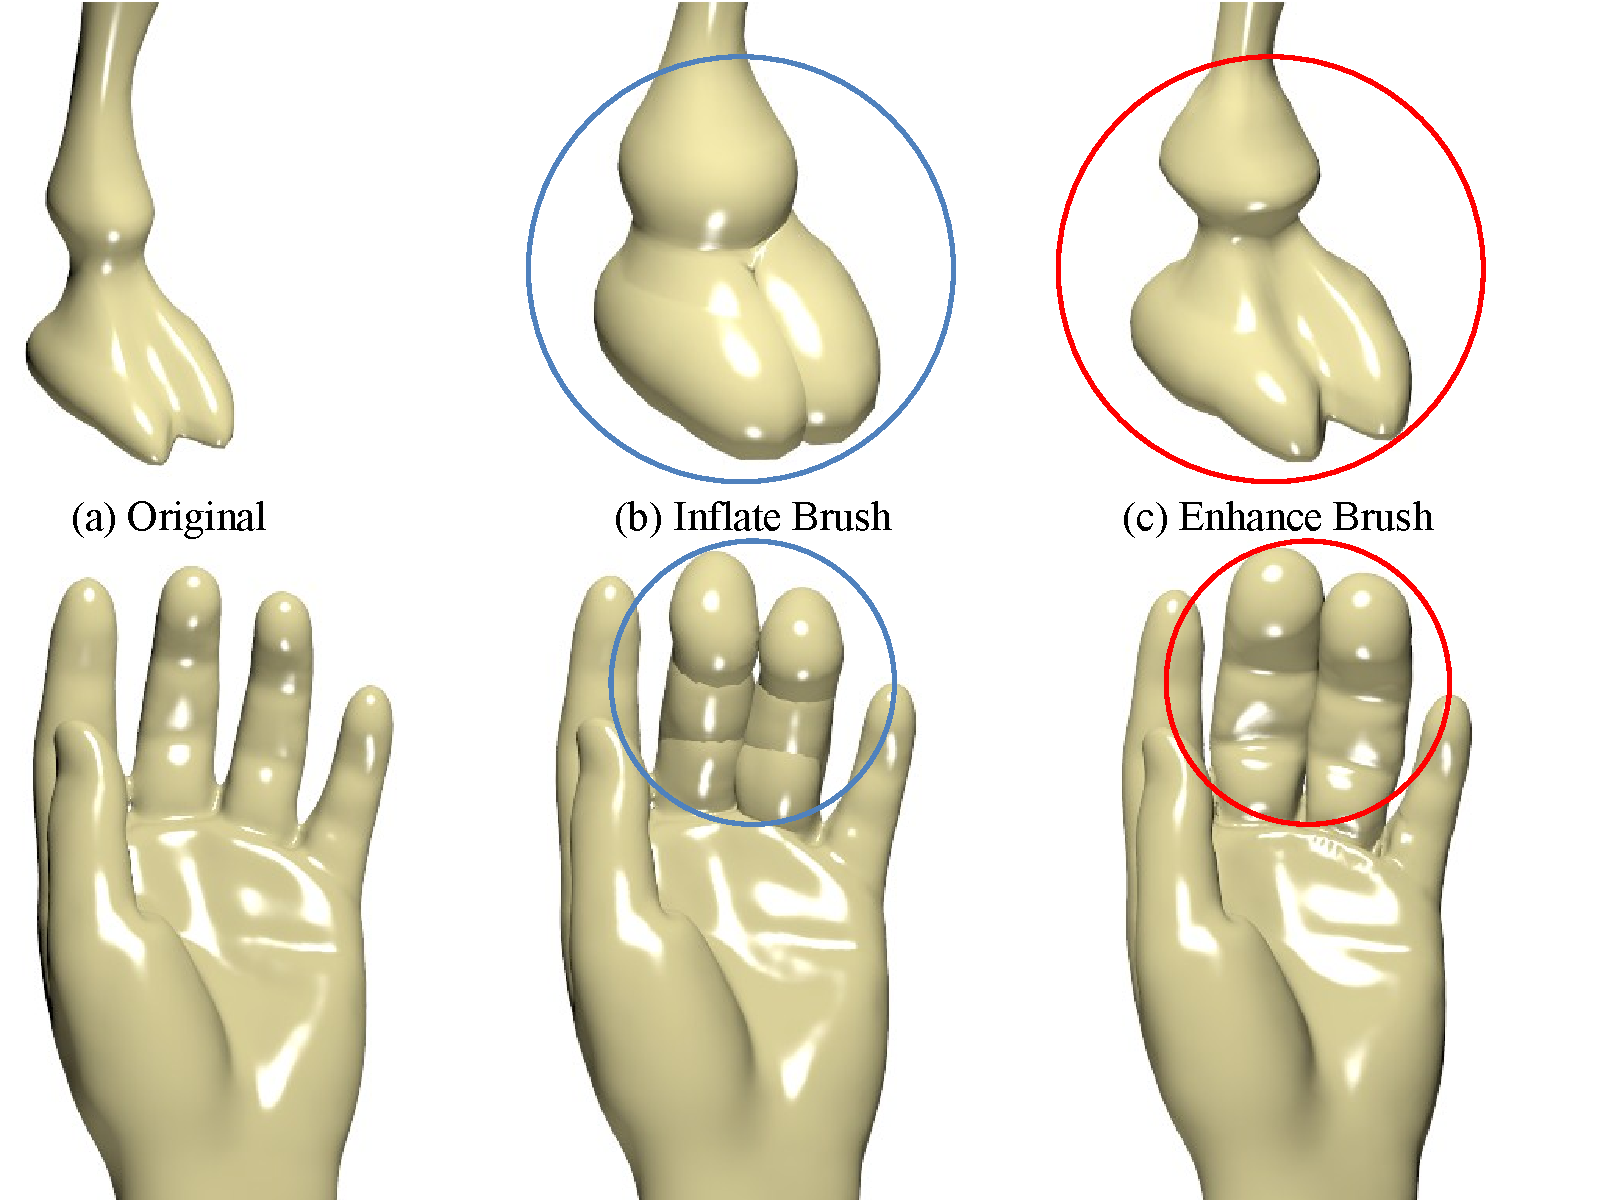
\includegraphics[width=1\columnwidth]{images/sculpt_brush}

\caption{\label{fig:Sculpt_Brush}Top row: (a) Leg Camel, (b) Inflate brush
for leg into blue circle, (c) Enhance curvature brush for leg into
red circle. Bottom row: (a) Hand, (b) Inflate brush for fingers into
blue circle, (c) Enhance curvature brush for fingers in red circle.}
\end{figure}


\begin{figure}
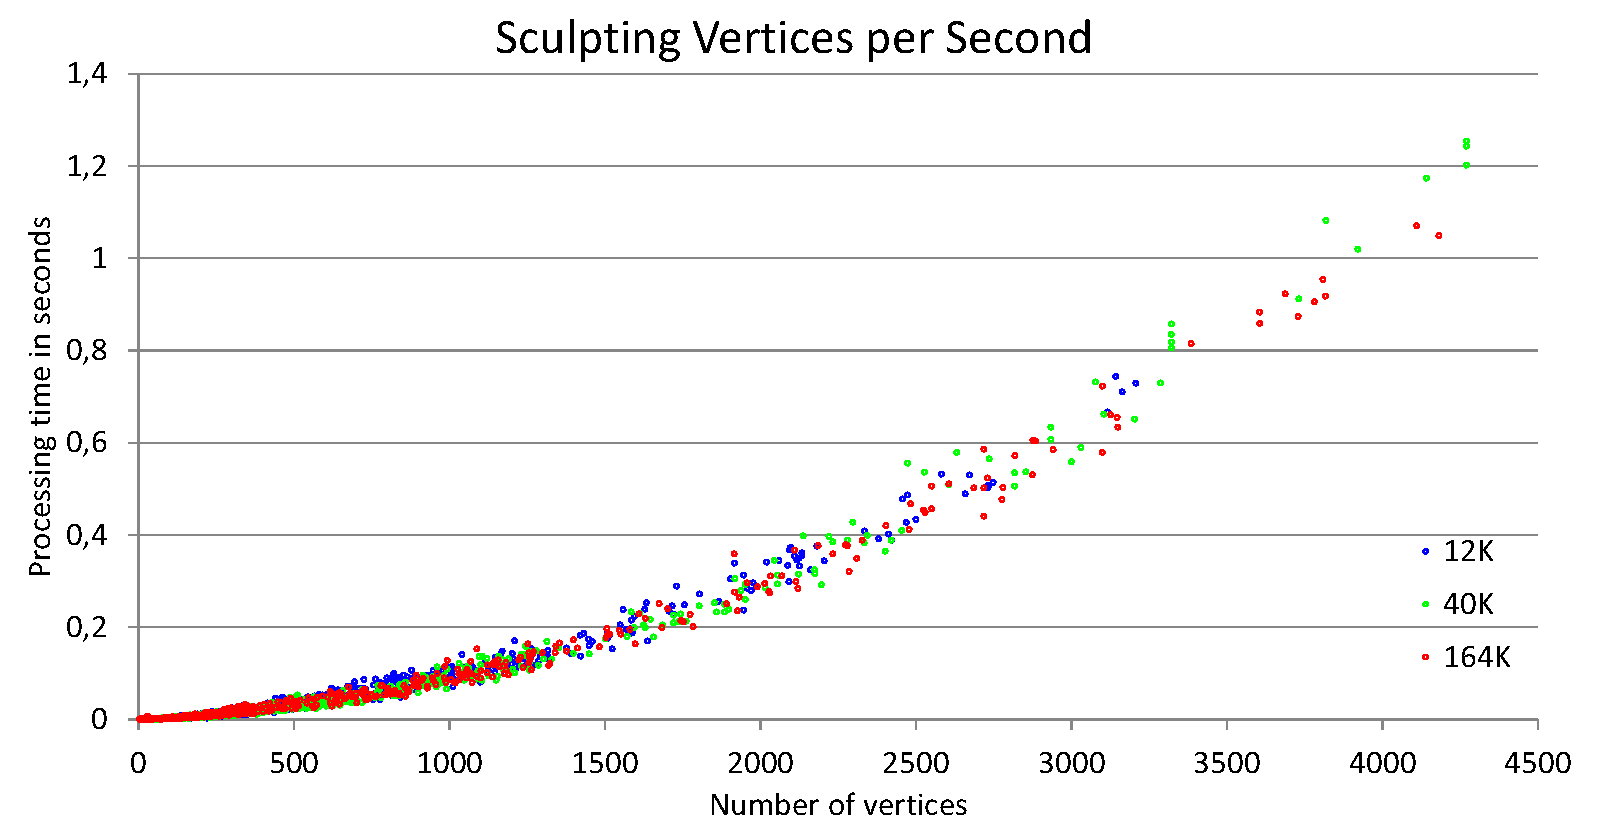
\includegraphics[width=1\columnwidth]{images/verts_per_second_sculpt}

\caption{\label{fig:Performance-sculpt}Performance of our dynamic curvature
enhance brush in terms of vertices sculpted per second. Three models
with 12K, 40K, 164K vertices used for sculpting in real time.}
\end{figure}


\begin{figure}
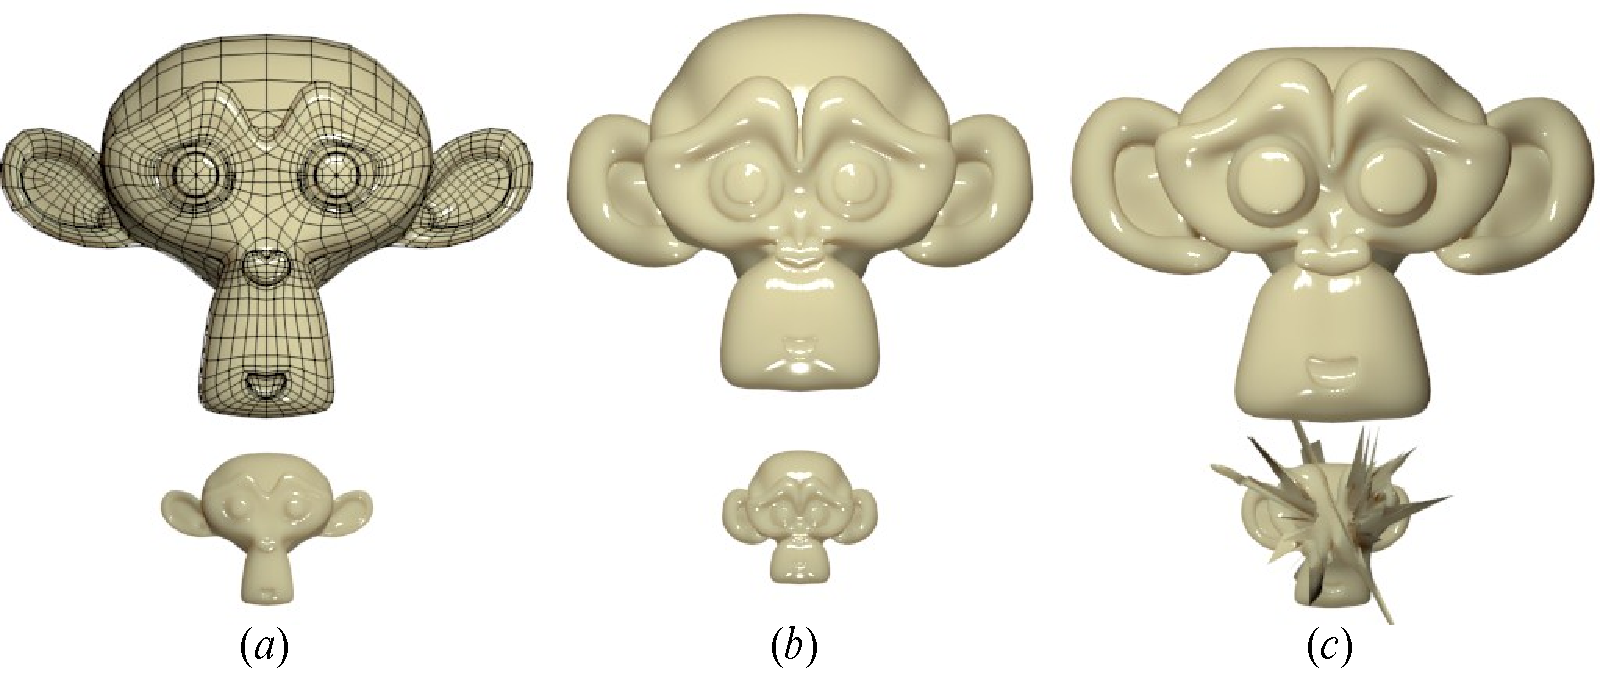
\includegraphics[width=1\columnwidth]{images/monkey}

\caption{\label{fig:(a)Monkey}(a) Top row: Original model scaled by 4. Bottom
row: Original Model (b) Top and bottom row: enhancing with Normalized-TQLBO
$\lambda=-50$ (c) Top and bottom row: enhancing with TQLBO $\lambda=-50$.}
\end{figure}


\begin{figure*}[t]
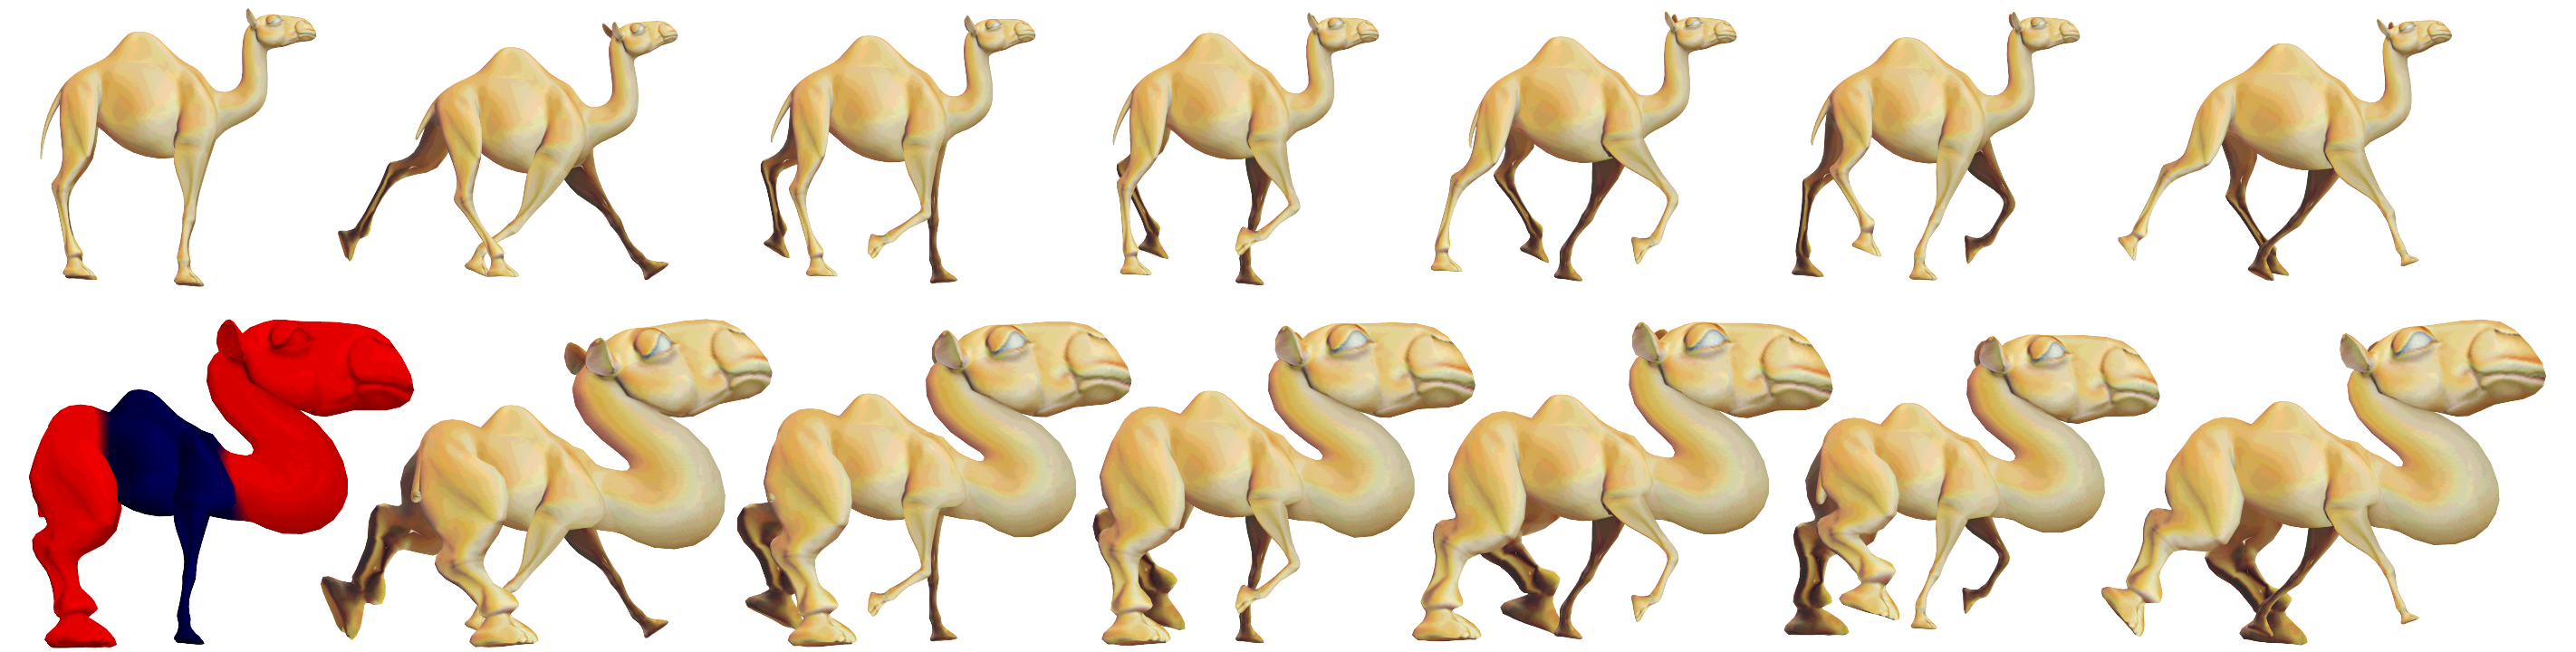
\includegraphics[width=1\textwidth]{images/camello_walk2}

\caption{\label{fig:Animated_Camell}Our method is pose insensitive. The enhanced
for the different poses are similar in terms of shape. Top row: Original
walk cycle camel model. Bottom row: Curvature enhancing with weight
vertex group, $\lambda=-400$ and $2$ iterations. }
\end{figure*}



\subsection{Implementation\label{sub:Implementation}}

Our method was implemented how a modifier for modeling and brush for
sculpting on the Blender software \cite{blender} with C and C++.
Working with Blender allowed us to test the method interactively with
others as Catmull-Clark, weight vertex groups and sculpting system
in Blender.

To improve performance, we worked with the Blender mesh struct calculating
all possible data each time visiting each triangle or quad and adding
to its corresponding index in a list that stored the sum of the Laplacian
weights of the ring, in this way only had to visit two times the list
of faces of the mesh list and the two times the list of the edges
if the mesh was not closed. To brush sculpting mode was necessary
to create a list that will map the index of the selected vertices
to a list from 1 to N where N is the number of vertices selected and
the number of rows in the linear system to solve, with this drastically
reduced the calculations should make working with the tool allowing
real-time. In the construction of our Laplacian matrix were blocked
at vertices having faces areas or lengths edges with value zero that
can cause spikes and bad results.

The matrix \ref{eq:TQLBO_Simple_Matrix} is sparse since the number
of neighbors per vertex corresponding to the number of data per row
is small compared to the total number of vertices in the mesh. To
solve the linear system equation \ref{eq:Lineal_System_with_wp} was
used OpenNL which is a a library for solving sparse linear system.


\section{Conclusion and future work\label{sec:Conclusion-and-future}}

We present an extension of the Laplace Beltrami operator for triangles
and quads that can work in production environments without conversion
that provides results similar to those obtained by working only with
triangles or quads. 

We introduced a new way to perform enhancement silhouettes in a mesh
for modeling or sculpted in a few steps allows the modification of
the curvature of a model while maintaining its overall shape. We introduce
a new method of modeling and show some of its possible uses. We show
that the method behaves in predictable ways which facilitate the learning
process, it also showed that the method works well with isometric
transformations opening the possibility of introducing it on the stages
of animation.

We demonstrate that this tool serves to work in the early stages in
which are used coarse models to permit modifying the curvature generated
by the Catmull-Clark subdivision surfaces, avoiding the edition of
the vertices to have only to change a few parameters.

As future work we would like to analyze theoretically the relationship
between the Catmull-Clark subdivision surfaces and Laplacian smoothing
because in some cases can produce very similar results. But the subdivision
surface is a fast method thereby reducing computation times for calculate
curvature in the mesh.


\section*{Acknowledgments}

We wold like to thank Eduardo Romero and CIM\&LAB Computer Imaging
\& Medical Applications Laboratory for their support of our research. 

This work was supported in part by the Blender Foundation, Google
Summer of code program at 2012. 

Livingstone elephant model is provided courtesy of INRIA and ISTI
by the AIM@SHAPE Shape Repository. Hand model is courtesy of the FarField
Technology Ltd. Camel model by Valera Ivanov is licensed under a Creative
Commons Attribution 3.0 Unported License.

\bibliographystyle{acmsiggraph/acmsiggraph}
\bibliography{template}
 
\end{document}
